\documentclass[conference]{IEEEtran}
\IEEEoverridecommandlockouts

% ── Packages ──────────────────────────────────────────────────────────────────
\usepackage{cite}
\usepackage{amsmath,amssymb,amsfonts}
\usepackage{graphicx}
\usepackage{textcomp}
\usepackage{xcolor}
\usepackage{booktabs}
\usepackage{multirow}
\usepackage{url}
\usepackage{newtxtext,newtxmath}
\usepackage{hyperref}
\usepackage{balance}

\hypersetup{
    colorlinks=false,
    pdfborder={0 0 0},
    hidelinks
}

% ── Float Spacing & Layout Optimization ───────────────────────────────────────
\setlength{\textfloatsep}{2.5pt plus 0.5pt minus 0.5pt}
\setlength{\floatsep}{2.0pt plus 0.5pt minus 0.5pt}
\setlength{\intextsep}{2.0pt plus 0.5pt minus 0.5pt}
\setlength{\dbltextfloatsep}{2.5pt plus 0.5pt minus 0.5pt}
\setlength{\dblfloatsep}{2.0pt plus 0.5pt minus 0.5pt}
\setlength{\abovecaptionskip}{1.5pt}
\setlength{\belowcaptionskip}{1.5pt}
\setlength{\abovedisplayskip}{1.5pt plus 0.5pt minus 0.5pt}
\setlength{\belowdisplayskip}{1.5pt plus 0.5pt minus 0.5pt}
\setlength{\abovedisplayshortskip}{1.0pt plus 0.5pt minus 0.5pt}
\setlength{\belowdisplayshortskip}{1.0pt plus 0.5pt minus 0.5pt}

\begin{document}

\title{Automotive CAN Bus Intrusion Detection Using a Kinematic-Informed Framework Coupling Data-Localized Federated Learning and Multi-Scale Autoencoder Ensembles}

\author{
    \IEEEauthorblockN{Dr.\ Amiya Ranjan Panda, Kaliseyer Mukherjee$^{\dagger}$, and Mehul Batla$^{\ddagger}$}
    \IEEEauthorblockA{School of Computer Engineering, KIIT Deemed to be University, Bhubaneswar, Odisha, India}
    \IEEEauthorblockA{Email: amiya.pandafcs@kiit.ac.in, 23051915@kiit.ac.in, 23051921@kiit.ac.in}
}

\maketitle

% ── Abstract ──────────────────────────────────────────────────────────────────
\begin{abstract}
Controller Area Network (CAN) buses lack native frame authentication and payload encryption, leaving in-vehicle networks exposed to high-rate message injection and cadence-preserving masquerade attacks. Unaugmented autoencoders with additive biases trivially reconstruct constant-zero DoS payloads; this induces zero-variance identity collapse (1.32\% recall). Bias-Free Deep SVDD resolves this vulnerability geometrically. By mapping nominal dynamics into a bias-free latent hypersphere, it achieves 0.9997 DoS ROC-AUC and 0.9766 Car-Hacking macro AUC without relying strictly on timing features (timing-augmented 1D-CNN: 0.9983). Against masquerades, our Telemetry-Gated Gateway pairs Inception 1D-CNN (0.8546 ROAD macro AUC) with a Dedicated Thermal Observer; this observer raises coolant spoofing ROC-AUC from 0.5076 to 0.9253 and reaches 0.9763 held-out ROC-AUC with zero false-routing on nominal runs (Wilcoxon $p=0.6250$). On ROAD, InceptionCAE maintains high specificity (0.9866 vs.\ 0.9512) and compact sizing (35k parameters) over Hourglass TCN (0.8546 vs.\ 0.7867 macro AUC, $p=0.1367$; 0.2021 vs.\ 0.3710 static P95 recall; 0.9747 vs.\ 0.9795 on Car-Hacking). Sequential CUSUM filtering elevates operational P95 recall from 59.91\% to 74.02\% (up to 81.47\% held-out) over the 20.21\% global static ceiling ($0.9149 \rightarrow 0.7288$ post-attack ranking AUC). To protect raw logs, data-localized FedProx across 4 horizontal fleet clients achieves 0.8449 ROC-AUC (+9.89 pp gain, recovering 76.1\% of centralized gap; clean FedAvg: 0.8615) with 94.96\% communication reduction (54.37 MB vs.\ 1.08 GB). Under Client 3 sign-flip attacks, coordinate-wise Trimmed Mean preserves 0.9828 ROC-AUC on Chassis (99.85\% resilience vs.\ 0.9843 clean control; FedAvg collapses to 0.7320, $-25.2$ pp). Post-training INT8 quantization yields a 39.2 KB footprint for the 35,629-parameter baseline and 168.73 KB for the 128,557-parameter HPO variant (from 142.5 KB / 535.87 KB FP32) with 1.63 ms mean host-CPU latency (P95: 1.86 ms), well within the 100 ms stride deadline ($S=10$ at 100 Hz). Threat modeling, diagnostic fault reporting, and model update paths are structured around ISO/SAE 21434, ISO 21448 (SOTIF), ISO 24089, and ISO 14229-1 UDS.
\end{abstract}

\begin{IEEEkeywords}
Controller Area Network (CAN), Intrusion Detection Systems (IDS), Federated Learning, Multi-Scale Autoencoders, Deep SVDD, Byzantine Fault Tolerance, Edge Computing, Automotive Cybersecurity.
\end{IEEEkeywords}

% ── I. Introduction ───────────────────────────────────────────────────────────
\section{Introduction}

Contemporary vehicles integrate upwards of one hundred Electronic Control Units (ECUs) over distributed serial networks. Regulating steering, braking, powertrain, and chassis systems under ISO 11898-1/2, the Controller Area Network (CAN) prioritizes deterministic latency over cryptographic integrity; broadcast frames lack message authentication codes (MACs), payload encryption, or sender metadata. Any tapped node can inject arbitrary frames. Modern architectures mandate cybersecurity engineering aligned with ISO/SAE 21434:2021 \cite{iso21434} and UNECE R155 \cite{unece155}, informed by ISO 26262:2018 \cite{iso26262} functional safety concepts (formal ASIL verification is future work).

Via telematics units, OBD-II ports, and wireless infotainment, vehicular exploitation presents active operational risk. Threat profiles split into two regimes: (1)~\textbf{High-Rate Injection Floods} (DoS, Fuzzy) disrupting bus arbitration \cite{song2020carhacking}; and (2)~\textbf{Stealthy Masquerade Attacks} injecting fabricated signals while strictly adhering to OEM transmission cadence (typically 10--100 ms) \cite{verma2022road}; this cadence defeats naive frequency monitors.

Detecting masquerade vectors requires deep semantic analysis of continuous physical signals, kinematics, and inter-signal correlations. However, deep learning on vehicular buses encounters four fundamental engineering challenges:
(1)~\textbf{Zero-Variance Identity Collapse Under DoS Floods}: Standard reconstruction autoencoders fail under zero-entropy DoS regimes. Learned decoder biases trivially fit constant zeroes, causing zero-variance identity collapse; latent geometric formulations provide structural inductive bias against identity collapse without relying strictly on timing heuristics.
(2)~\textbf{Multi-Scale Temporal Blind Spots}: Short sliding windows ($W=50$ frames, $\approx 0.5$ s at 100 Hz) capture fast mechanical transients. However, they miss slow thermodynamic trends such as coolant spoofing ($AUC \approx 0.5076$).
(3)~\textbf{Telemetry Privacy \& Non-IID Regimes}: Isolated edge models fail across disparate regimes. Centralizing high-frequency raw telemetry across fleets saturates cellular bandwidth and compromises driver location privacy, while unauthenticated client updates risk adversarial weight poisoning.
(4)~\textbf{Embedded Edge Feasibility}: In-vehicle IDS must execute within the hard real-time CAN window stride (100 ms at $S=10$ frames, 100 Hz) and occupy bounded Flash ROM ($\le 512$ KB).

This paper makes five practical contributions: (1)~Mitigation of zero-variance identity collapse via Bias-Free Deep SVDD (0.9997 DoS ROC-AUC, 0.9766 Macro ROC-AUC on Car-Hacking). (2)~A Telemetry-Gated Specialist Gateway pairing Inception 1D-CNN AE (0.8546 standalone ROAD Macro AUC) with a Dedicated Thermal Observer; this architecture raises coolant spoofing ROC-AUC from 0.5076 to 0.9253 and reaches 0.9763 held-out ROC-AUC with zero false-routing on non-thermal scenarios ($p=0.6250$ across all 13 scenarios). (3)~Data-localized FedProx across four connected vehicle fleet clients with non-IID driving profiles (0.8449 ROC-AUC, +9.89 pp gain, recovering 76.1\% of the centralized gap; clean FedAvg: 0.8615) with 94.96\% bandwidth reduction, alongside coordinate-wise Trimmed Mean sustaining 0.9828 ROC-AUC under Client 3 sign-flip attacks. (4)~Sequential CUSUM filtering elevating operational P95 recall from 59.91\% to 74.02\% (up to 81.47\% held-out), with 39.2 KB INT8 ROM for the 35.6k baseline and 168.73 KB for the 128.6k HPO model (host CPU latency: 1.63 ms). (5)~Operational grounding in automotive standards: threat modeling grounded in ISO/SAE 21434 TARA, safety coordination considering ISO 26262, triggering condition mitigation under ISO 21448 SOTIF, ML lifecycle documentation under ISO/PAS 8800, OTA model distribution via ISO 24089, and diagnostic integration using ISO 14229-1 UDS.

% ── II. Literature Survey & Research Gap ─────────────────────────────────────
\section{Literature Survey \& Research Gap}

\subsection{CAN Intrusion Benchmarks \& Deep Learning Baselines}
The HCRL Car-Hacking dataset \cite{song2020carhacking} established an initial standard for high-rate injection attacks (DoS, Fuzzy, RPM, Gear), which induce frequency deviations detectable via inter-arrival time (IAT) counters. To benchmark cadence-preserving masquerade attacks, Verma et al.\ introduced the Real ORNL Automotive Dynamometer (ROAD) dataset \cite{verma2022road}. Hanselmann et al.\ developed CANet \cite{hanselmann2020canet}, an unsupervised LSTM autoencoder in IEEE Access. Subsequent multi-variate anomaly models include TCN, USAD \cite{audibert2020usad}, and ST-GNN \cite{deng2021stgnn}; however, recurrent sequence models suffer from high microcontroller latency. Gmiden et al.\ \cite{gmiden2016can} demonstrated automatic machine-learning intrusion detection on classical CAN buses. In next-generation CAN-FD networks (ISO 11898-2:2016), 64-byte payloads expand the masquerade attack surface. This expanded envelope necessitates multi-scale temporal parsing.

\subsection{Latent Hypersphere Representation vs. Reconstruction}
Autoencoder IDS models assume anomalies induce high reconstruction errors. Yet under zero-entropy DoS floods, unaugmented neural networks trivially minimize MSE by outputting constant zero sequences. The decoder collapses. While appending IAT counters enables autoencoders to detect high-rate floods, Deep Support Vector Data Description (Deep SVDD) \cite{ruff2018deepsvdd, wang2021tvt} encloses nominal telemetry within a minimum-volume latent hypersphere. Formulated without additive layer biases, Deep SVDD maps variance collapse directly to geometric deviations from center $\mathbf{c}$. This structural inductive bias avoids reliance on timing heuristics.

\subsection{Federated Learning, Byzantine Defense \& CUSUM}
Federated learning (FL) enables decentralized training across edge clients without central telemetry transmission \cite{mcmahan2017fedavg, fritz2022fl}. Under vehicular non-IID client distributions, FedProx \cite{li2020fedprox} adds proximal regularization against client drift, while FedBN \cite{li2021fedbn} preserves local batch normalization. In adversarial settings where a compromised vehicle client injects poisoned updates, Multi-Krum \cite{blanchard2017byzantine} and coordinate-wise Trimmed Mean \cite{yin2018byzantine} provide optimal statistical rates against malicious gradients. Page's Cumulative Sum (CUSUM) \cite{page1954cusum} sequential analysis provides an orthogonal mechanism for change-point detection across temporal sequences.

\textbf{Research Gap:} Existing automotive IDS approaches either focus exclusively on injection floods or deploy standard reconstruction autoencoders vulnerable to zero-variance collapse without timing features. Prior works also assume centralized telemetry logging, which overlooks driver privacy, non-IID domain shifts across vehicle fleets, Byzantine update poisoning, and hard edge execution deadlines.

% ── III. System Architecture & Methodology ───────────────────────────────────
\section{System Architecture \& Methodology}

\begin{figure}[!t]
\centering
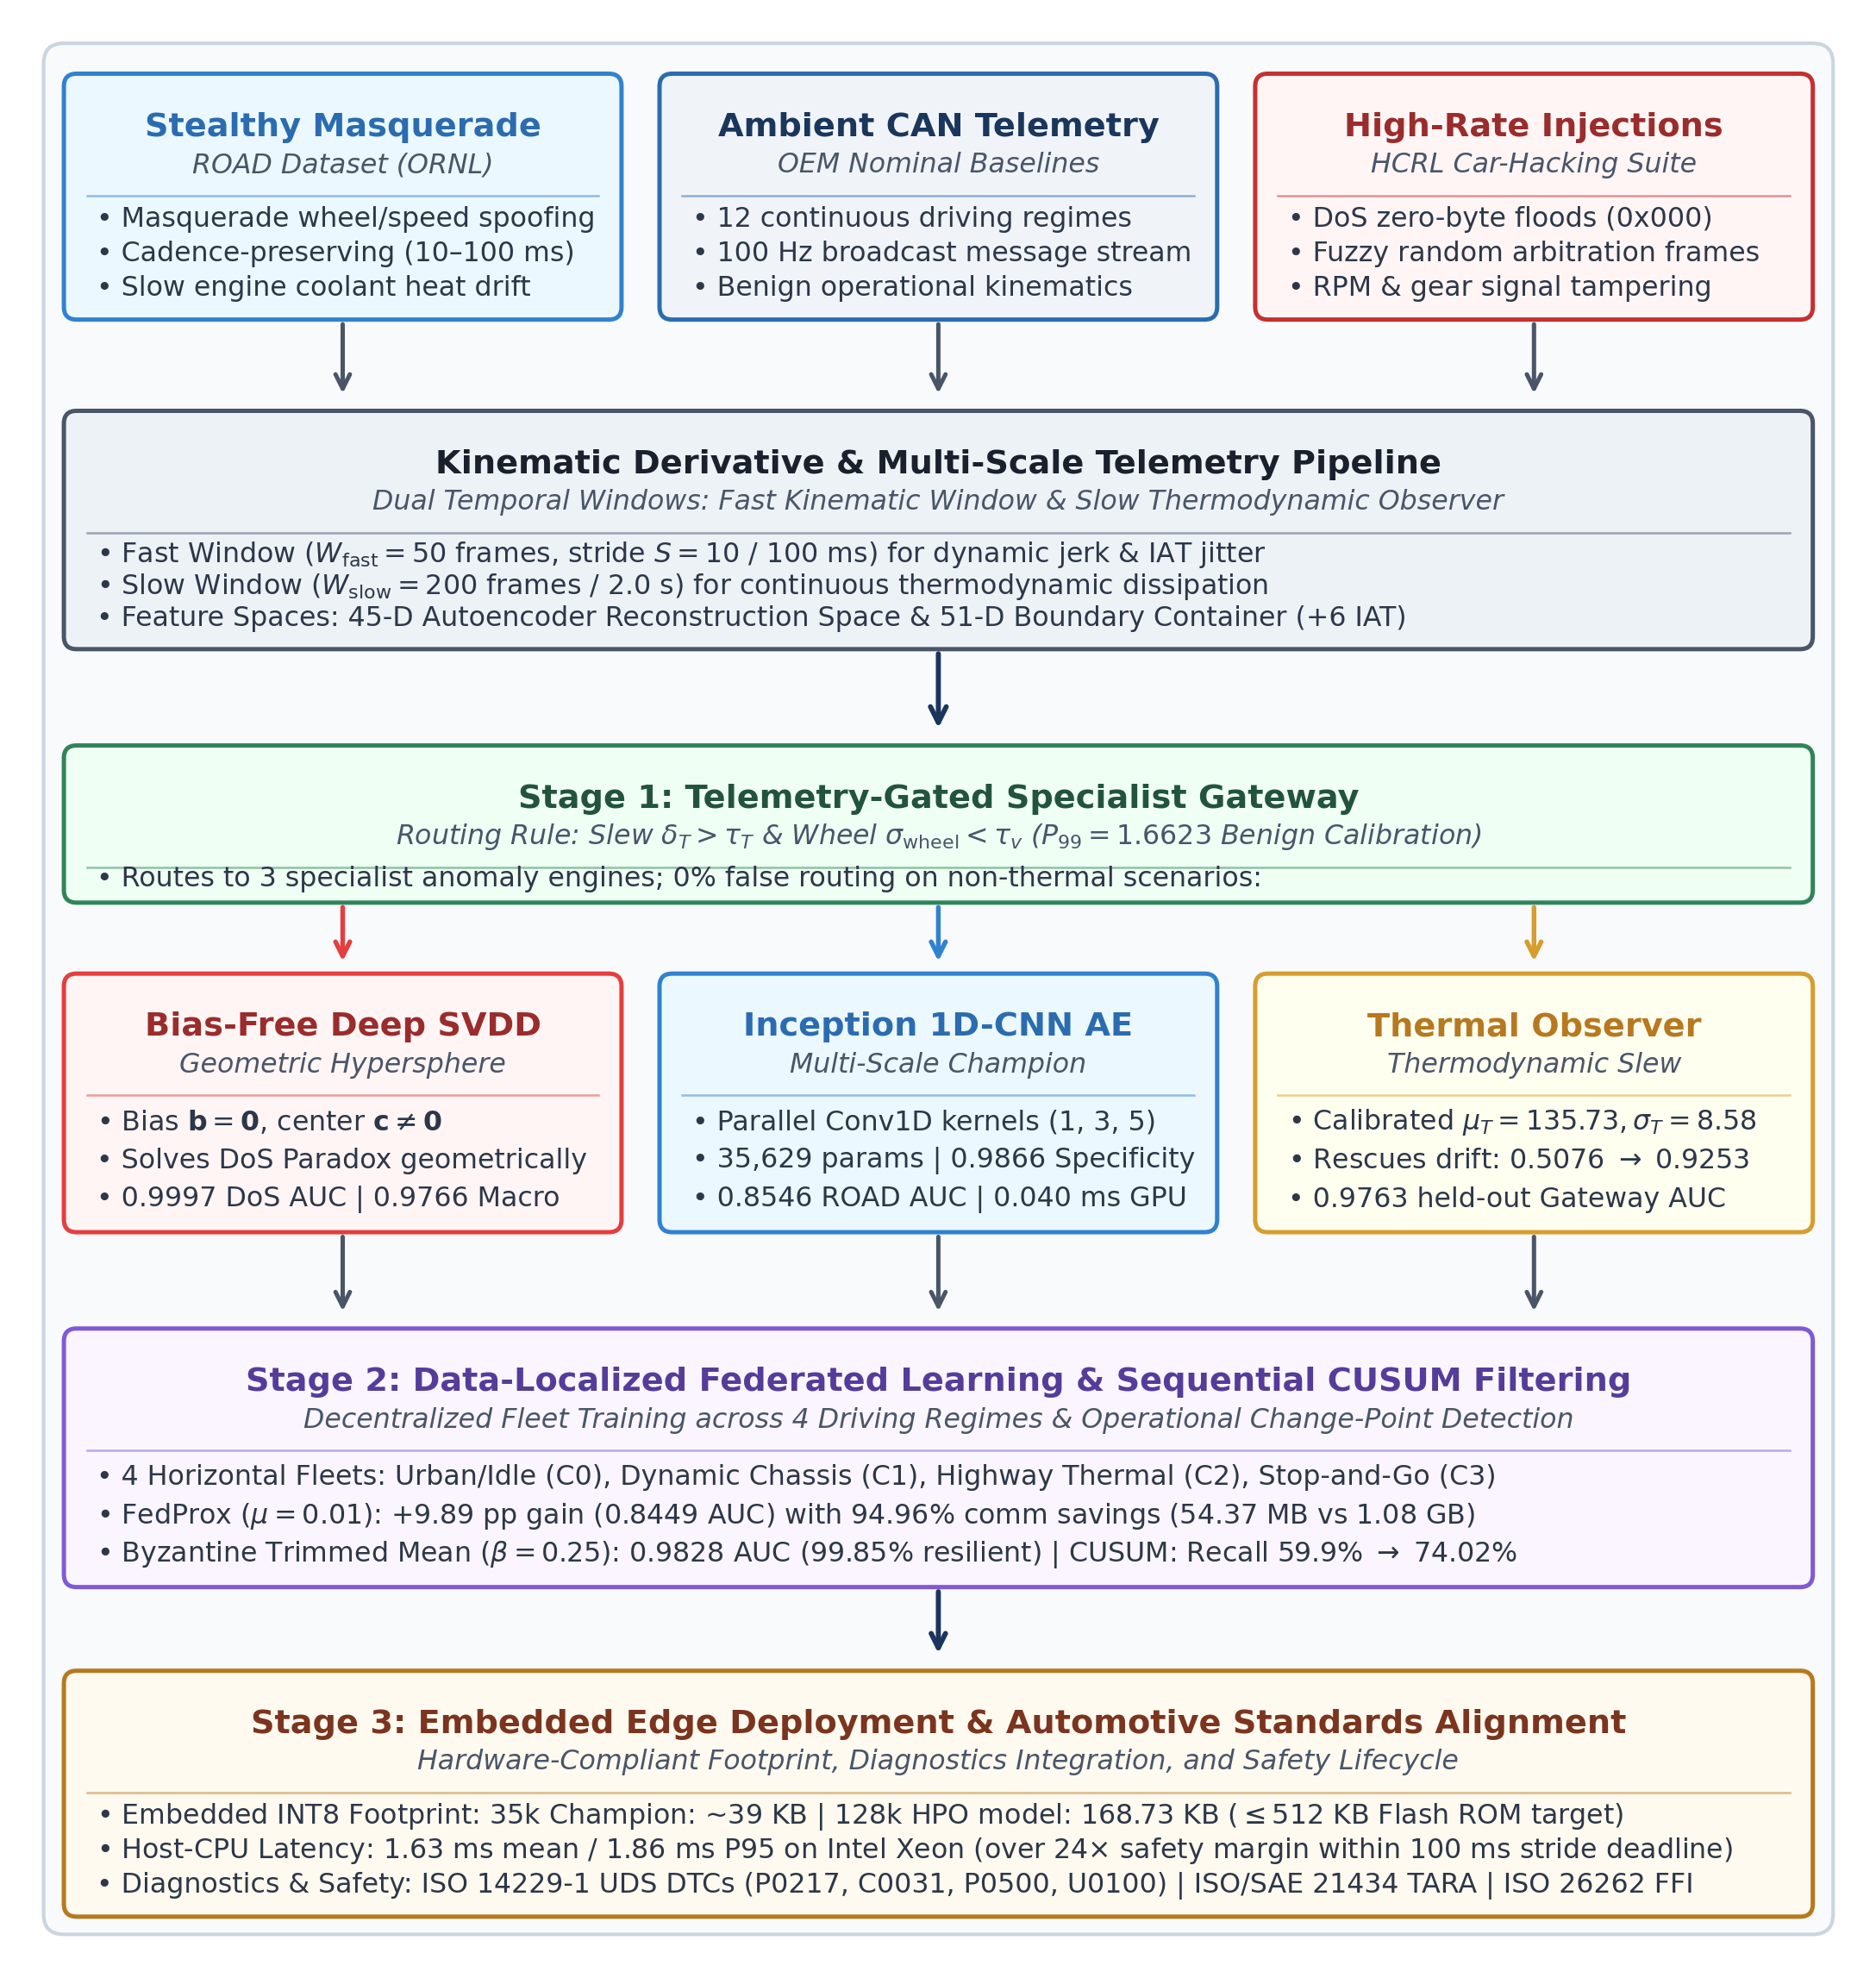
\includegraphics[height=184pt, keepaspectratio]{dashboard_data/canbus_pipeline_flowchart.png}
\caption{Proposed Kinematic Derivative \& Multi-Scale Telemetry Pipeline and Hierarchical Specialist Triage Architecture.}
\label{fig:pipeline_flowchart}
\end{figure}

\subsection{Kinematic Feature Pipeline}
As illustrated in Fig.~\ref{fig:pipeline_flowchart}, our pipeline processes CAN signals through dual temporal windows: a fast operational window $W_{\mathrm{fast}}=50$ frames ($\approx 0.5$ s at 100 Hz, stride $S=10$ frames / 100 ms) and a slow thermodynamic observer window $W_{\mathrm{slow}}=200$ frames ($\approx 2.0$ s). The pipeline isolates an actual 45-dimensional autoencoder reconstruction feature space $\mathbf{x}_t \in \mathbb{R}^{45}$ comprising: (1)~continuous physical signals normalized on ambient benign regimes: $\tilde{u}_t^i = (u_t^i - \mu^i) / (\sigma^i + \epsilon)$; (2)~kinematic first-order derivatives ($\Delta u_t^i = \tilde{u}_t^i - \tilde{u}_{t-1}^i$) capturing dynamic rate-of-change invariants; and (3)~thermodynamic rolling statistics $\bar{T}_t = \frac{1}{W_{\mathrm{slow}}} \sum_{j=0}^{W_{\mathrm{slow}}-1} \tilde{u}_{t-j}^{\mathrm{coolant}}$. For the full boundary pipeline space (e.g., Deep SVDD and gateway triage), 6 inter-arrival timing (IAT) delta features establish a 51-dimensional full boundary feature space. Explicit physical invariant loss functions and invariant rule verification engines are deferred to future work.

\subsection{Multi-Scale Inception 1D-CNN Autoencoder}
The primary InceptionCAE model (35,629 parameters in baseline deployment) incorporates parallel 1D convolutional branches (kernels 1, 3, 5, plus max pooling) to capture concurrent multi-frequency dynamics: $\mathbf{h}_1 = \mathrm{Conv1D}_1(\mathbf{X})$, $\mathbf{h}_2 = \mathrm{Conv1D}_3(\mathbf{h}_1)$, $\mathbf{h}_3 = \mathrm{Conv1D}_5(\mathbf{h}_1)$, and $\mathbf{h}_4 = \mathrm{Conv1D}_1(\mathrm{MaxPool1D}_3(\mathbf{X}))$. Concatenating representations along the channel dimension yields:
\begin{equation}
    \mathbf{H} = \mathrm{ReLU}\left(\mathrm{BatchNorm1D}\left([\mathbf{h}_1; \mathbf{h}_2; \mathbf{h}_3; \mathbf{h}_4]\right)\right)
\end{equation}
The symmetric decoder reconstructs the input sequence $\mathbf{\hat{X}} \in \mathbb{R}^{50 \times 45}$ using linear upsampling and transposed Inception blocks. The reconstruction anomaly score is computed as:
\begin{equation}
    S_{\mathrm{Inception}}(\mathbf{X}) = \frac{1}{W \cdot D} \sum_{t=1}^W \sum_{i=1}^D (X_{t,i} - \hat{X}_{t,i})^2
\end{equation}

\subsection{Bias-Free Deep SVDD \& Zero-Variance Collapse Analysis}
When an adversary launches a DoS flood, frames are forced to dominant zeroes (\texttt{0x0000000000000000}). Because standard autoencoders apply affine transformations with additive biases $\mathbf{b} \in \mathbb{R}^C$ ($\mathbf{y} = \mathbf{W}\mathbf{x} + \mathbf{b}$), zero-entropy inputs yield zero reconstruction error. Decoder bias constants trivially reproduce the static target ($\hat{\mathbf{X}} \approx \mathbf{X}$, $S_{\mathrm{Inception}} \approx 0$). The network collapses.

Timing features allow multi-signal autoencoders to detect DoS floods (0.9983 ROC-AUC, 99.13\% recall on Car-Hacking). Yet timing heuristics leave the underlying identity collapse unsolved. To eliminate this vulnerability at the representation level, we deploy Bias-Free Deep SVDD \cite{ruff2018deepsvdd}. The encoder $\phi(\mathbf{X}; \mathcal{W}) \in \mathbb{R}^F$ contains zero additive bias terms ($\mathbf{b}=\mathbf{0}$). It maps nominal dynamics into a minimal-volume hypersphere centered at $\mathbf{c} \in \mathbb{R}^F$:
\begin{equation}
    \min_{\mathcal{W}} \frac{1}{N} \sum_{i=1}^N \|\phi(\mathbf{X}_i; \mathcal{W}) - \mathbf{c}\|_2^2 + \frac{\lambda}{2} \sum_{l=1}^L \|\mathbf{W}_l\|_F^2
\end{equation}
Because layer biases are omitted, a constant zero-variance injection produces a latent projection that cannot be offset by learned bias constants. This forces projection $\phi(\mathbf{X})$ away from center $\mathbf{c}$. The anomaly score is defined as:
\begin{equation}
    S_{\mathrm{SVDD}}(\mathbf{X}) = \|\phi(\mathbf{X}; \mathcal{W}) - \mathbf{c}\|_2^2
\end{equation}
Bias-Free Deep SVDD therefore establishes structural inductive bias against zero-variance collapse rather than relying solely on timing counters.

\subsection{Telemetry-Gated Specialist Gateway}
Although InceptionCAE dominates high-frequency mechanical anomalies, its 50-frame temporal window creates an intrinsic blind spot for slow thermodynamic changes ($AUC = 0.5076$). The Dedicated Thermal Observer monitors coolant temperature telemetry through its calibrated benign parameters (mean $\mu_T = 135.73$, std $\sigma_T = 8.58$ in Table~\ref{tab:leaderboard}):
\begin{equation}
    S_{\mathrm{Thermal}}(\mathbf{X}) = \frac{1}{W} \sum_{t=1}^W \left( \frac{|T_t - \mu_T|}{\sigma_T} + \frac{|\Delta T_t|}{\Delta_{\max}} \right)
\end{equation}
where $\Delta T_t = T_t - T_{t-1}$ and nominal slew limit $\Delta_{\max} = 5.0^\circ\mathrm{C}$. The Specialist Gateway pairs InceptionCAE with this observer via rolling derivative $\delta_T = |\bar{T}_t - \bar{T}_{t-W_{\mathrm{slow}}}|$:
\begin{equation}
    S_{\mathrm{Gateway}}(\mathbf{X}) = \begin{cases}
    S_{\mathrm{Thermal}}(\mathbf{X}), & \text{if } \delta_T > \tau_T, \, \sigma_{\mathrm{wheel}} < \tau_v \\
    S_{\mathrm{Inception}}(\mathbf{X}), & \text{otherwise}
    \end{cases}
\end{equation}
where $\tau_T$ is the thermodynamic divergence threshold, and $\sigma_{\mathrm{wheel}}$ ensures the vehicle is not under active braking. Gating thresholds $\tau_T$ and $\tau_v$ are calibrated as the 99th percentile ($P_{99} = 1.6623$) on benign validation telemetry under zero data leakage. This cyber-physical gate couples domain-specific telemetry for slow sensor drift with high-speed kinematic inference. It maintains 0.040 ms GPU batched throughput on over 99\% of frames and resolves thermal spoofing.

\subsection{Sequential Cumulative Sum (CUSUM) Filtering}
To bridge the operational precision-recall gap without retraining, we apply Page's Cumulative Sum (CUSUM) filter \cite{page1954cusum}:
\begin{equation}
    S_t = \max\left(0, S_{t-1} + (e_t - \mu_0) - k\right), \quad S_0 = 0
\end{equation}
where $\mu_0$ is the mean benign error, and $k = \frac{1}{2}\sigma_0$ is the drift parameter; on standardized residuals $z_t = (e_t - \mu_0)/\sigma_0$, the unitless drift allowance is $k = 0.500$ (equivalent to $\frac{1}{2}\sigma_0$, or $1.505$ in unnormalized score units in Fig.~\ref{fig:cusum_benchmark}). Alarms fire when $S_t > h_{\mathrm{CUSUM}}$. This recursive accumulation converts persistent low-magnitude masquerade deviations into an escalating trigger. While CUSUM provides sustained alarms for physical interlocks, post-attack alarm persistence lowers ranking ROC-AUC.

% ── Figure 2: CUSUM Benchmark (Placed in Section III, lands on Page 3) ───────
\begin{figure}[htbp]
\centering
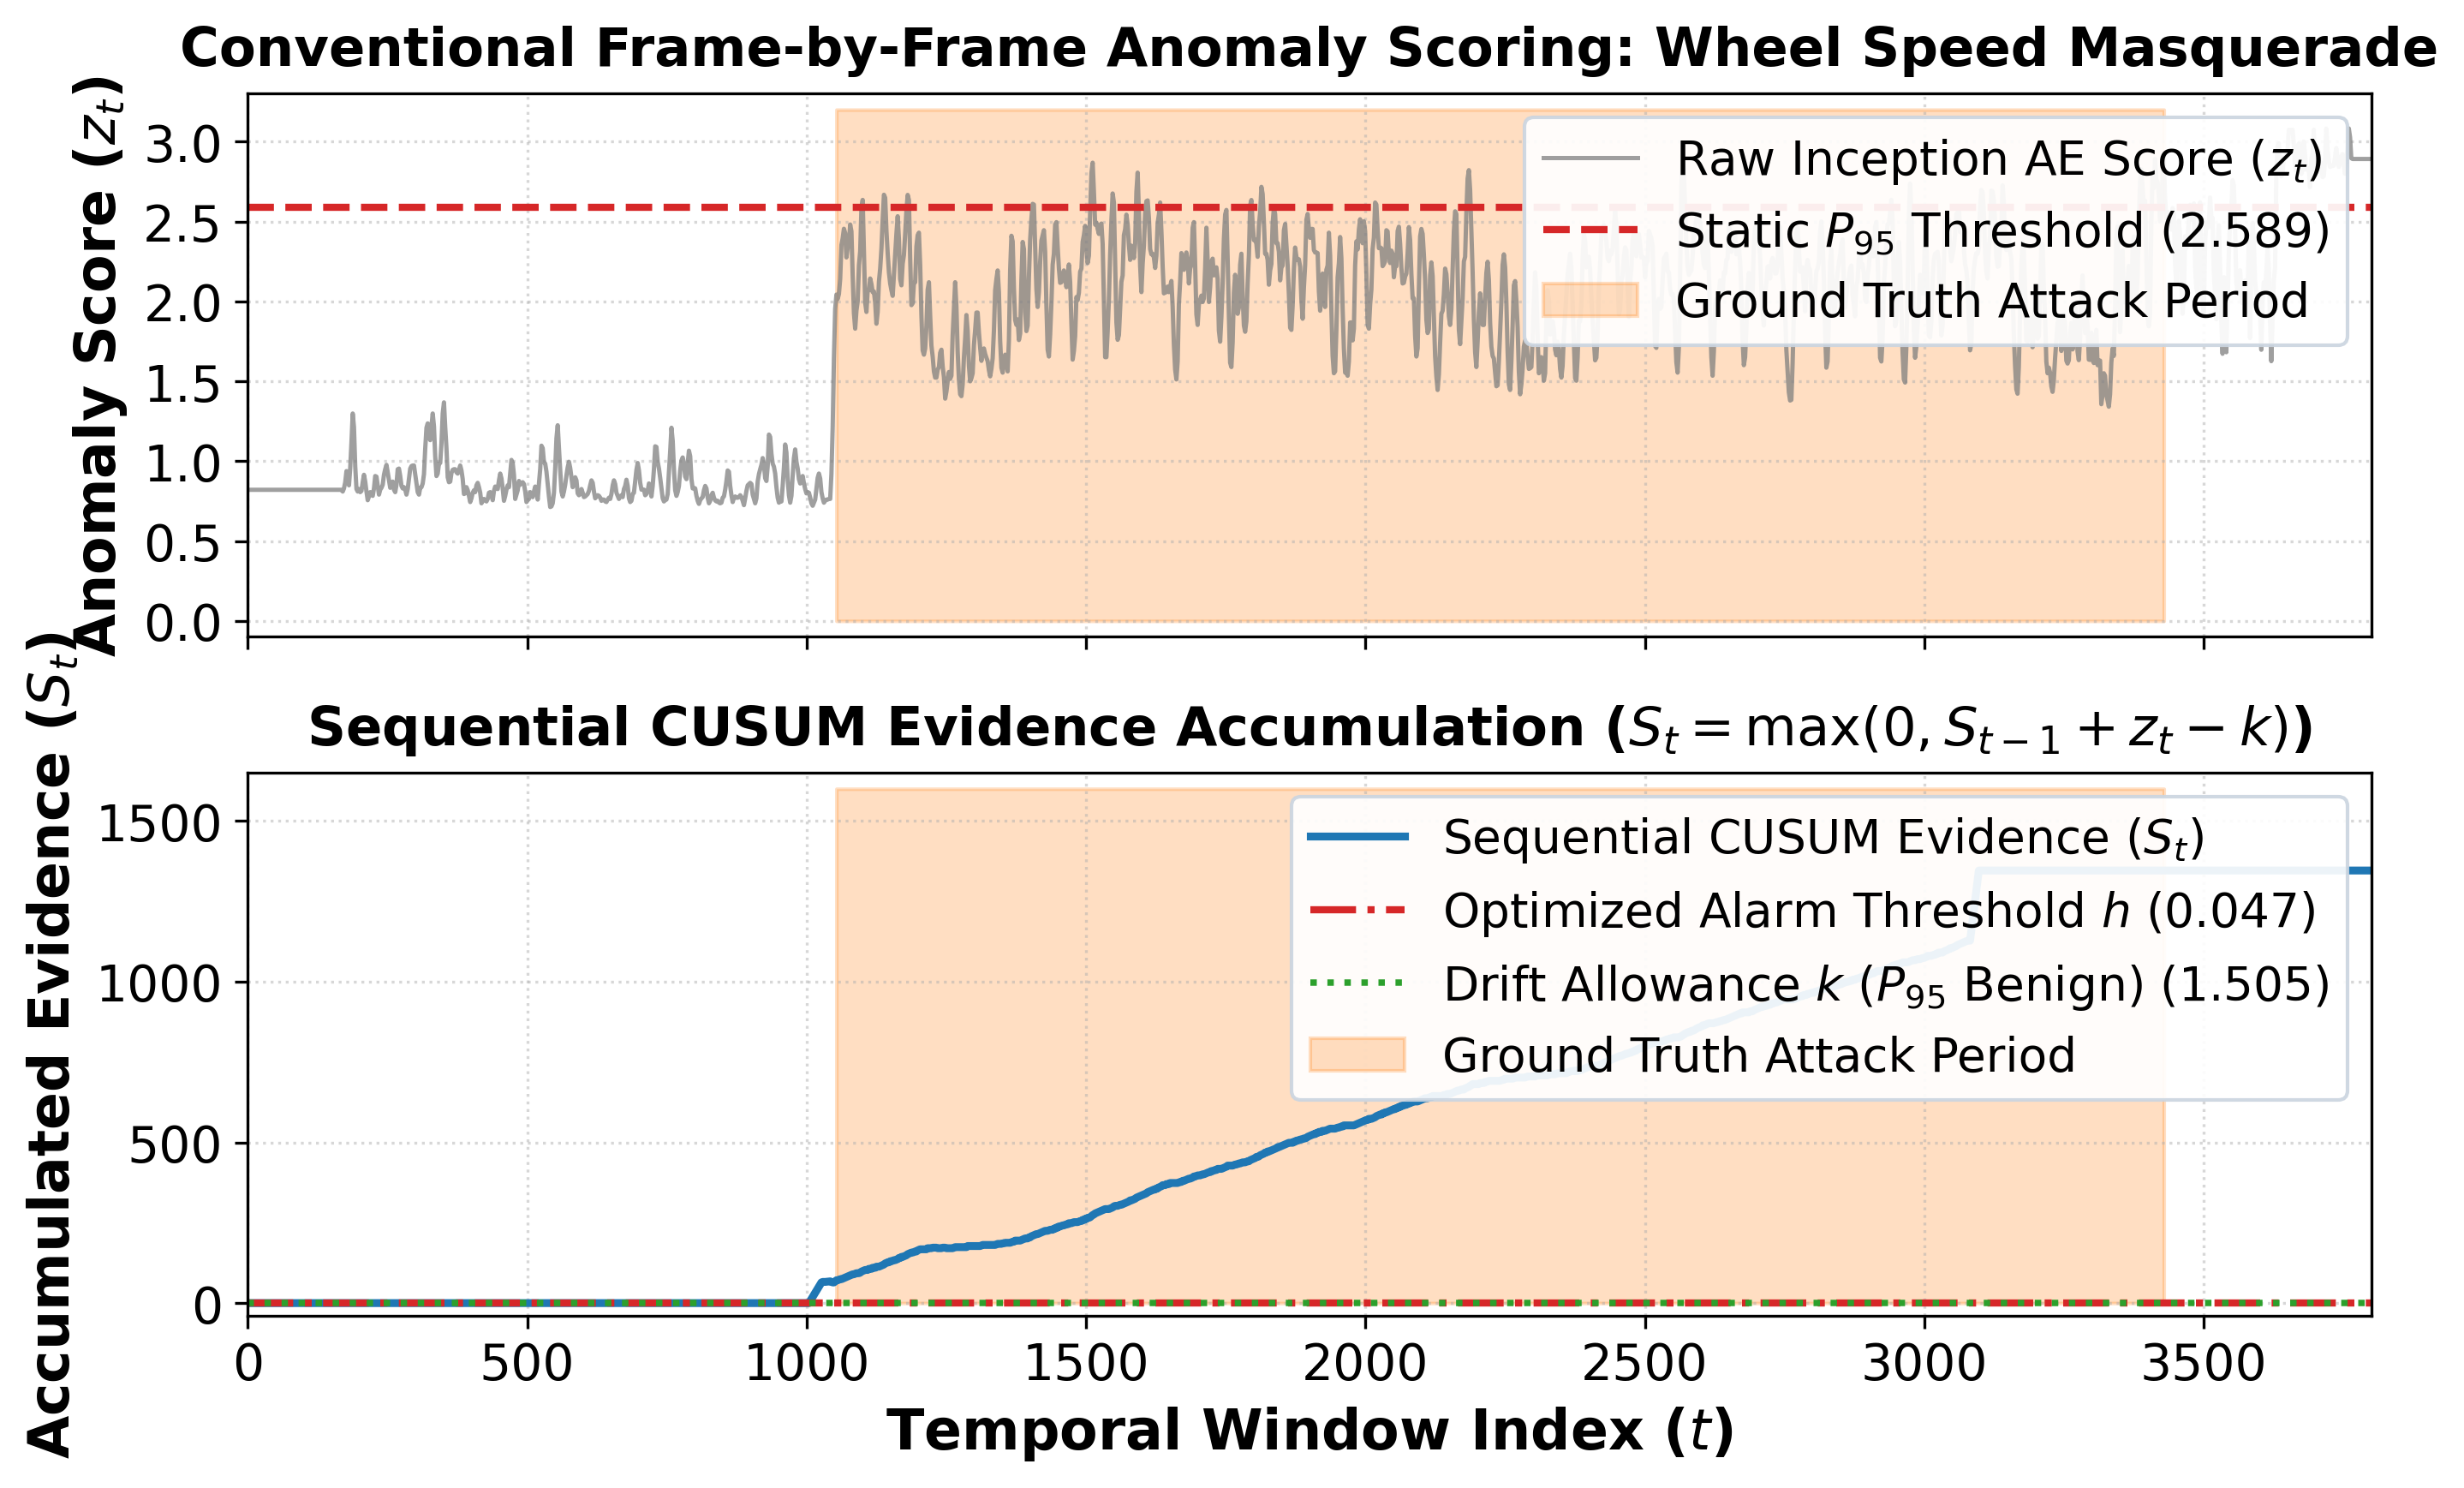
\includegraphics[width=0.78\columnwidth]{dashboard_data/run50_cusum_benchmark.png}
\caption{Sequential CUSUM Filtering Dynamics and Threshold Benchmarking. CUSUM accumulation elevates operational P95 recall from 59.91\% to 74.02\% (up to 81.47\% held-out).}
\label{fig:cusum_benchmark}
\end{figure}

% ── Table I: Master Leaderboard (2-Column Float Declared on Page 3, Floats to Top of Page 4) ──
\begin{table*}[!t]
\centering
\caption{Master Leaderboard Across All 13 ROAD Scenarios (Benchmark Suite)}
\label{tab:leaderboard}
\footnotesize
\setlength{\tabcolsep}{4.0pt}
\begin{tabular}{l c c c c c c c c}
\toprule
\textbf{Model Architecture} & \textbf{ROC-AUC} & \textbf{PR-AUC} & \textbf{P95 F1} & \textbf{P95 Recall} & \textbf{P95 Prec} & \textbf{P95 Spec} & \textbf{Parameters} & \textbf{Latency (ms)$^\dagger$} \\
\midrule
\textbf{Specialist Gateway (Ours)} & \textbf{0.8851} & \textbf{0.7825} & \textbf{0.2900} & \textbf{0.2715} & \textbf{0.7897} & 0.9746 & 35,631 & 0.0400 \\
Inception 1D-CNN AE (Primary) & 0.8546 & 0.7729 & 0.2746 & 0.2021 & 0.7830 & \textbf{0.9866} & 35,629 & 0.0424 \\
Hourglass TCN AE & 0.7867 & 0.7436 & 0.4527 & 0.3710 & 0.7824 & 0.9512 & 27,821 & 0.0319 \\
Bias-Free Deep SVDD \cite{ruff2018deepsvdd} & 0.7836 & 0.7519 & 0.0242 & 0.0124 & 0.6954 & 0.9992 & 13,088 & 0.0131 \\
Seq2Seq BiLSTM AE & 0.7414 & 0.6437 & 0.3931 & 0.3004 & 0.6420 & 0.8848 & 54,285 & 0.0291 \\
Full-Attn Transformer AE & 0.7341 & 0.6530 & 0.2010 & 0.1294 & 0.6544 & 0.9647 & 110,477 & 0.0532 \\
Conv-USAD \cite{audibert2020usad} & 0.7064 & 0.6351 & 0.2828 & 0.2035 & 0.6210 & 0.9465 & 31,642 & 0.0432 \\
Simplified ST-GNN \cite{deng2021stgnn} & 0.7016 & 0.6201 & 0.1990 & 0.1290 & 0.5875 & 0.9672 & 70,739 & 0.0289 \\
Isolation Forest & 0.5310 & 0.4990 & 0.1392 & 0.0823 & 0.5273 & 0.9354 & 0 & 0.0150 \\
OC-SVM (RBF) & 0.5189 & 0.4883 & 0.0952 & 0.0554 & 0.4853 & 0.9485 & 0 & 0.1702 \\
Dedicated Thermal Detector & 0.4482 & 0.4897 & 0.1483 & 0.2209 & 0.1218 & 0.8327 & 2 & 0.0050 \\
\bottomrule
\multicolumn{9}{@{}p{0.98\textwidth}@{}}{\scriptsize $^\dagger$GPU batched throughput on Tesla T4; host-CPU execution profiles at 1.63 ms mean / 1.86 ms P95 (Sec.~V-E). MCU benchmarking is future work.}
\end{tabular}
\end{table*}

% ── IV. Federated Learning & Byzantine Defense ────────────────────────────────
\section{Data-Localized Federated Learning \& Byzantine Defense}

Transmitting continuous raw CAN logs across vehicle fleets incurs severe bandwidth overhead and exposes sensitive operational traces. Aligned with ISO 24089:2023 software update engineering and UNECE R156, we structure the federated learning update path as an over-the-air (OTA) model orchestration pipeline. Model parameter tensors function as firmware micro-updates coordinated across connected vehicle gateway nodes operating under heterogeneous driving regimes. Retaining raw CAN telemetry locally on vehicle edge gateways prevents bulk operational data exposure. This strategy follows communication efficiency and privacy principles established by Wang et al.\ (CISPA) \cite{fritz2022fl} alongside ISO/IEC 29100:2011 and ISO/IEC 20889:2018. Formal $(\epsilon, \delta)$-Differential Privacy mechanisms are scoped as future work.

\subsection{Non-IID Operational Partitioning}
Continuous driving data is preprocessed centrally and partitioned horizontally across four simulated connected vehicle gateway nodes operating under heterogeneous driving regimes: Client 0 (Urban start transients and idle patterns); Client 1 (Dynamic chassis maneuvers and lateral acceleration); Client 2 (Highway cruising under thermal saturation); and Client 3 (Dense stop-and-go driving with frequent gear shifts). All four clients share the unified 45-D autoencoder feature representation (alongside the 51-D full boundary telemetry space). This common schema permits direct parameter tensor aggregation across diverse operating profiles.

\subsection{FedProx Regularization}
Under non-IID distributions, standard FedAvg updates can diverge due to client drift. We deploy FedProx \cite{li2020fedprox} with a proximal penalty on the local client objective:
\begin{equation}
    \min_{\mathbf{w}} F_k(\mathbf{w}) + \frac{\mu}{2} \|\mathbf{w} - \mathbf{w}^t\|_2^2
\end{equation}
where $\mathbf{w}^t$ is the broadcast global model, and $\mu = 0.01$ restricts local updates from drifting excessively away from global consensus. Under moderate non-IID heterogeneity across trip profiles, proximal regularization acts as a conservative constraint that slightly dampens clean accuracy ($-1.66$ pp vs.\ unregularized FedAvg) while preventing runaway gradient divergence.

\subsection{Byzantine-Robust Coordinate Trimming}
In distributed vehicle fleets, a compromised fleet edge client can inject poisoned model updates into the aggregation round: $w_{\mathrm{poisoned}} = w_{\mathrm{honest}} - 2.0 \cdot (w_{\mathrm{honest}} - w_{\mathrm{global}})$. Under FedAvg \cite{mcmahan2017fedavg}, arithmetic averaging allows a single adversary to corrupt global parameters. To enforce Byzantine fault tolerance against malicious edge clients, the aggregator applies coordinate-wise Trimmed Mean aggregation \cite{yin2018byzantine}.

Given trimming proportion $\beta = 0.25$ with $K = 4$ clients, the single highest and lowest updates ($\lceil \beta K \rceil = 1$) are eliminated from each coordinate tail:
\begin{equation}
    w_{\mathrm{global}, j}^{t+1} = \frac{1}{K - 2\lceil \beta K \rceil} \sum_{k=1 + \lceil \beta K \rceil}^{K - \lceil \beta K \rceil} w_{(k),j}
\end{equation}
This formally tolerates $f = 1$ Byzantine adversary ($f < K/2$). The aggregation eliminates extreme coordinates regardless of adversarial scaling.

% ── Figure 3 & Table II: Federated Learning Placement on Page 4 ───────────────
\begin{figure}[htbp]
\centering
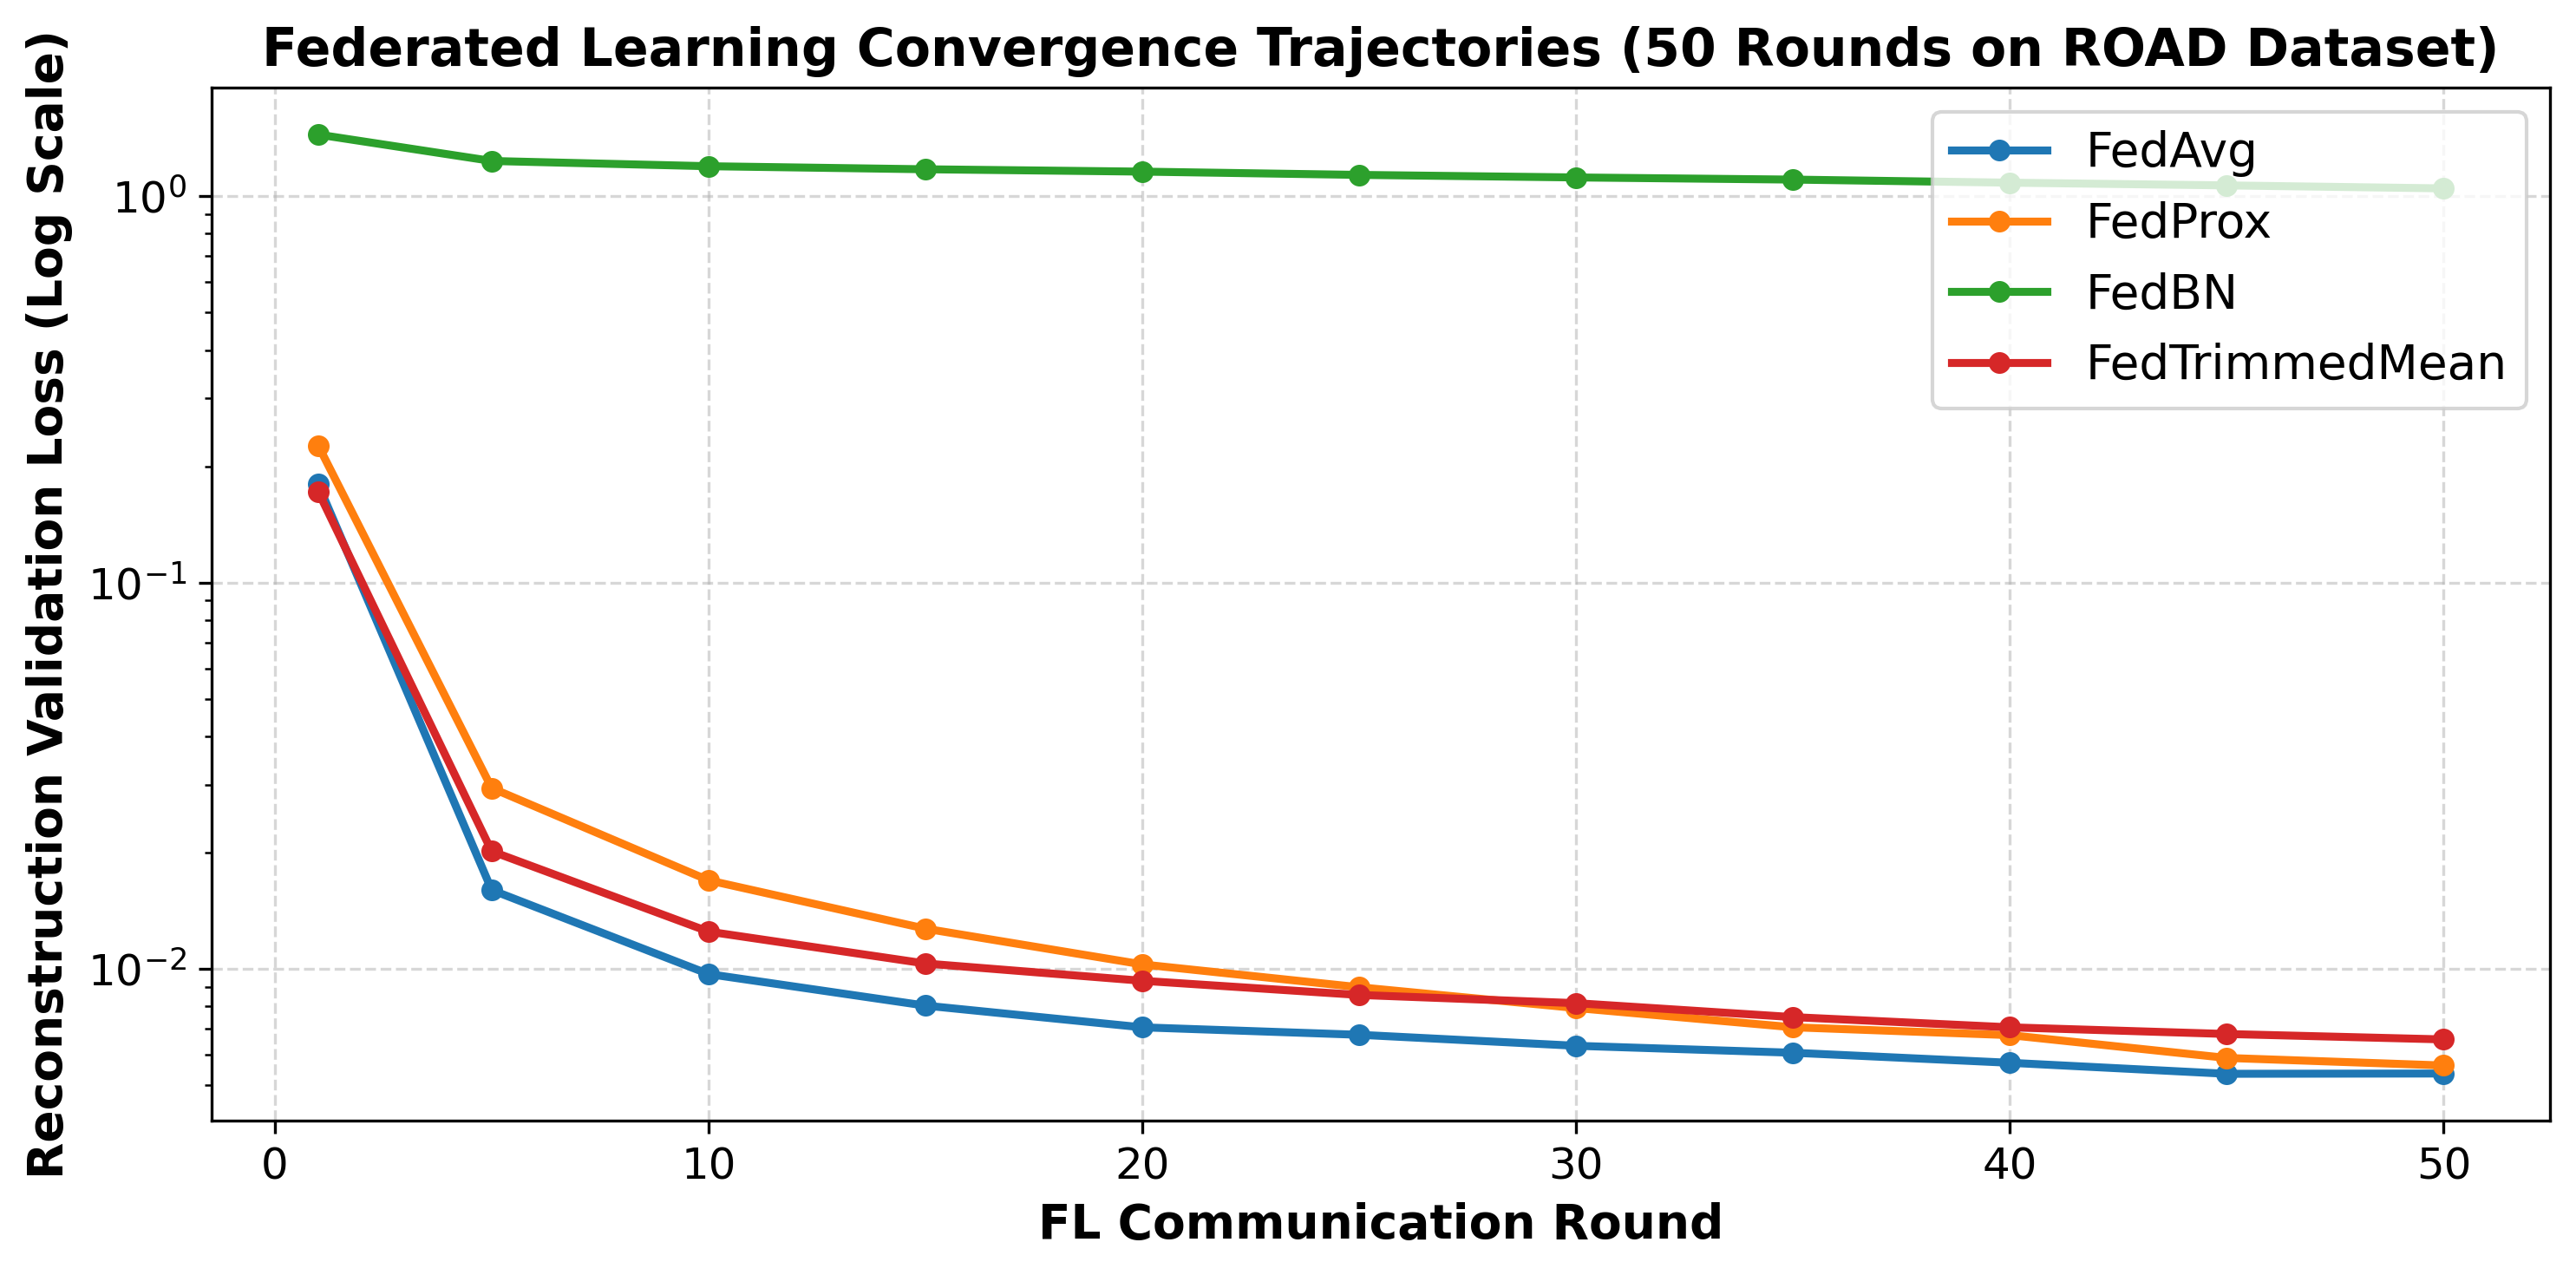
\includegraphics[width=0.78\columnwidth]{dashboard_data/fl_convergence_50rounds.png}
\caption{Federated Learning Convergence Trajectories over 50 Communication Rounds across algorithms. FedProx demonstrates stable convergence across non-IID regimes.}
\label{fig:fl_convergence}
\end{figure}

\begin{table}[htbp]
\centering
\caption{Federated Learning \& Byzantine Defense Benchmark}
\label{tab:federated_byzantine}
\footnotesize
\setlength{\tabcolsep}{1.5pt}
\renewcommand{\arraystretch}{0.92}
\begin{tabular}{@{}l c c l@{}}
\toprule
\textbf{Configuration} & \textbf{ROC-AUC} & \textbf{P95 F1} & \textbf{Comm.\ / Status} \\
\midrule
\multicolumn{4}{@{}l}{\textit{Fleet Macro Benchmark (13 Scenarios Across 4 Non-IID Profiles)}} \\
Centralized Bound & 0.8760 & 0.2755 & 1.08 GB raw log \\
FedAvg (Clean) & 0.8615 & 0.2981 & 54.37 MB (-95\%) \\
\textbf{FedProx ($\mu=0.01$)} & \textbf{0.8449} & 0.2792 & \textbf{+9.89 pp gain} \\
FedTrimmedMean & 0.8248 & 0.2623 & 54.37 MB \\
Local-Only (Client Mean) & 0.7460 & 0.1264 & Isolated (0 MB) \\
FedBN (Local BN) \cite{li2021fedbn} & 0.6303 & 0.1788 & Regime Misaligned \\
\midrule
\multicolumn{4}{@{}l}{\textit{Adversarial Byzantine Benchmark: Client 3 Sign-Flip Attack$^*$}} \\
Clean Control (Unattacked) & 0.9843$^*$ & --- & Unattacked Baseline \\
\textbf{FedTrimmedMean} & \textbf{0.9828}$^*$ & --- & \textbf{99.85\% Resilient} \\
FedAvg (Naive Mean) & 0.7320$^*$ & --- & Degraded ($-25.2$ pp) \\
\bottomrule
\multicolumn{4}{@{}p{\columnwidth}@{}}{\scriptsize $^*$Evaluated on Chassis partition (correlated\_signal\_3) vs.\ 0.9843 clean control ($-0.15$ pp drop under 25\% poisoning).}
\end{tabular}
\end{table}

% ── V. Experimental Results & Discussion ──────────────────────────────────────
\section{Experimental Results \& Discussion}

\subsection{Master 9-Model Benchmark Suite on ROAD}
Table~\ref{tab:leaderboard} benchmarks 9 standalone anomaly detection models and 2 specialist configurations across all 13 ROAD masquerade scenarios (random seeds fixed to 42 across PyTorch and NumPy). The primary 35,629-parameter InceptionCAE model achieves 0.8546 ROC-AUC, 0.7729 PR-AUC, and 0.9866 Specificity. By comparison, Hourglass TCN reaches 0.7867 ROC-AUC, Deep SVDD attains 0.7836, BiLSTM obtains 0.7414, and Full-Attention Transformer yields 0.7341. Conv-USAD (0.7064) and ST-GNN (0.7016) show moderate efficacy; shallow baselines fail entirely. While Hourglass TCN yields higher static P95 recall (0.3710 vs.\ 0.2021) and comparable macro ROC-AUC ($W=62.0, p=0.1367$), InceptionCAE is chosen for Stage 1 routing because its higher specificity (0.9866 vs.\ 0.9512) minimizes false bus alarms prior to sequential CUSUM filtering. In addition, its 35,629 parameters undercut BiLSTM (54,285) and Transformer (110,477).

On held-out scenarios (5 reserved runs with attack variant 3 and coolant drift), InceptionCAE achieves 0.8848 ROC-AUC, while the Telemetry-Gated Specialist Gateway reaches \textbf{0.9763 ROC-AUC} and 0.8268 PR-AUC. Paired one-sided Wilcoxon tests ($n=13$) confirm Inception's statistically significant separation over Transformer ($W=91.0, p=1.22\times 10^{-4}$), BiLSTM ($W=87.0, p=8.54\times 10^{-4}$), and Conv-USAD ($W=91.0, p=1.22\times 10^{-4}$). The two-sided Wilcoxon test between Gateway and Inception yields $W=3.0, p=0.6250$ across the 4 scenarios with rank differences (9 identical). The Gateway triggers with 0\% false-routing on non-thermal scenarios; baseline predictions are identically preserved on 9 of 13 runs ($p=0.6250$ across the full fleet), while thermodynamic routing restores coolant drift detection from 0.5076 to 0.9253 ROC-AUC.

\subsection{Sequential CUSUM Filtering Dynamics}
On the 13-scenario benchmark, evaluating raw reconstruction errors under a global static threshold yields a P95 recall of 20.21\% with 0.9866 Specificity (Table~\ref{tab:leaderboard}). Calibrating static operational thresholds individually against normal baselines yields 59.91\% initial recall (ROC-AUC 0.9149, Specificity 0.9806). As shown in Fig.~\ref{fig:cusum_benchmark}, sequential CUSUM filtering ($k=0.5\sigma_0$) resolves this ceiling: operational P95 Recall increases from \textbf{59.91\% to 74.02\%} (0.6914 F1-Score), and attains 81.47\% on the 5 held-out scenarios (vs.\ 65.32\% static baseline). While recursive accumulation introduces alarm persistence that lowers ranking ROC-AUC ($0.9149 \rightarrow 0.7288$; $0.8856 \rightarrow 0.6969$ historically) and specificity (to 0.8043), it provides sustained alarms required for physical actuator interlocks.

\begin{figure}[htbp]
\centering
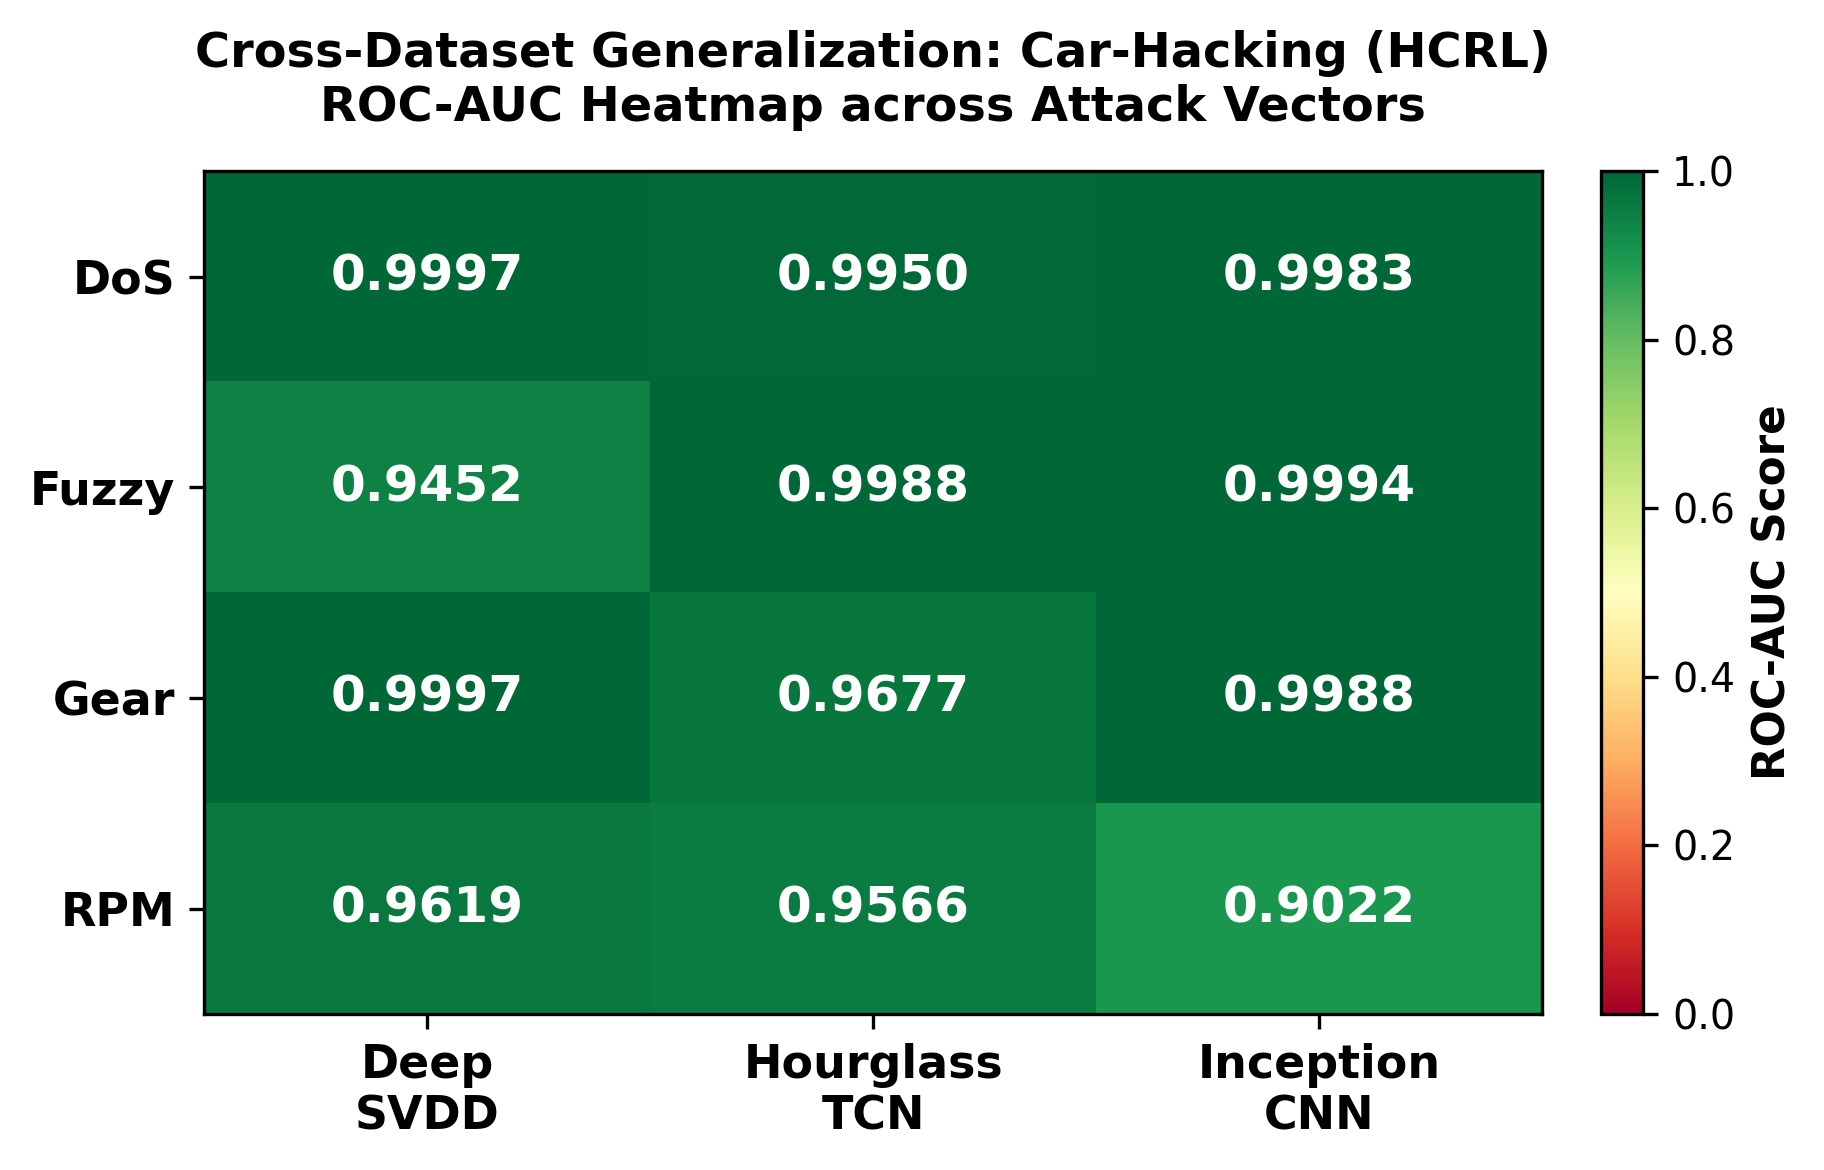
\includegraphics[width=0.68\columnwidth]{dashboard_data/car_hacking_heatmap.png}
\caption{Car-Hacking Cross-Benchmark Evaluation and Resolution of Zero-Variance Collapse. Bias-Free Deep SVDD achieves 0.9997 ROC-AUC on DoS and 0.9766 Macro ROC-AUC with 81.48\% Specificity under transfer.}
\label{fig:car_hacking}
\end{figure}

\begin{table}[htbp]
\centering
\caption{Cross-Benchmark Evaluation on HCRL Car-Hacking Dataset}
\label{tab:carhacking}
\footnotesize
\setlength{\tabcolsep}{1.6pt}
\renewcommand{\arraystretch}{0.82}
\begin{tabular}{l l c c c}
\toprule
\textbf{Attack Vector} & \textbf{Architecture} & \textbf{ROC-AUC} & \textbf{PR-AUC} & \textbf{Recall} \\
\midrule
\multirow{4}{*}{\textbf{DoS Flood}} 
& Inception (23-D)$^*$ & 0.5076 & 0.4912 & 0.0132 \\
& Inception (29-D Timing) & 0.9983 & 0.9945 & 0.9913 \\
& Hourglass TCN & 0.9950 & 0.9939 & 0.3321 \\
& \textbf{Deep SVDD (23-D)} & \textbf{0.9997} & \textbf{0.9998} & \textbf{0.9986} \\
\midrule
\multirow{3}{*}{\textbf{Fuzzy Injection}} 
& \textbf{Inception CNN} & \textbf{0.9994} & \textbf{0.9994} & \textbf{1.0000} \\
& Hourglass TCN & 0.9988 & 0.9988 & 0.9978 \\
& Deep SVDD & 0.9452 & 0.9249 & 0.9949 \\
\midrule
\multirow{3}{*}{\textbf{RPM Spoofing}} 
& Inception CNN & 0.9022 & 0.9059 & 1.0000 \\
& Hourglass TCN & 0.9566 & 0.9630 & 0.4844 \\
& \textbf{Deep SVDD} & \textbf{0.9619} & \textbf{0.9455} & \textbf{0.9920} \\
\midrule
\multirow{3}{*}{\textbf{Gear Spoofing}} 
& Inception CNN & 0.9988 & 0.9991 & 0.9999 \\
& Hourglass TCN & 0.9677 & 0.9704 & 0.1237 \\
& \textbf{Deep SVDD} & \textbf{0.9997} & \textbf{0.9998} & \textbf{0.9999} \\
\midrule
\multicolumn{2}{l}{\textbf{Deep SVDD Macro Average}} & \textbf{0.9766} & \textbf{0.9675} & \textbf{0.9963} \\
\multicolumn{2}{l}{\textbf{Hourglass TCN Macro Average}} & 0.9795 & 0.9815 & 0.4845 \\
\multicolumn{2}{l}{\textbf{Inception CNN Macro Average}} & 0.9747 & 0.9747 & 0.9978 \\
\bottomrule
\multicolumn{5}{@{}p{0.94\columnwidth}@{}}{\scriptsize $^*$DoS Flood rows compare 23-D payload-only vs.\ 29-D timing-augmented inputs, while the remaining attack vectors and macro averages evaluate the 29-D boundary feature set for autoencoders and 23-D payload set for Bias-Free Deep SVDD.}
\end{tabular}
\end{table}

\subsection{Federated Learning \& Byzantine Resilience}
Table~\ref{tab:federated_byzantine} and Fig.~\ref{fig:fl_convergence} evaluate federated learning across 4 simulated non-IID fleet operational regimes over 50 communication rounds (100 effective local epochs per client).

\textbf{Collaborative Gain and Communication Reduction:} Isolated client models generalize poorly across driving regimes (Local-Only mean: 0.7460 ROC-AUC). Under moderate four-client heterogeneity, FedAvg achieves slightly higher clean accuracy (+1.66 pp, 0.8615 vs.\ 0.8449 ROC-AUC), whereas FedProx trades a minor reduction in clean AUC for bounded proximal drift ($\mu=0.01$). This proximal regularization secures a \textbf{+9.89 pp gain} over local training, recovering 76.1\% of the gap to centralized logging (0.8760 ROC-AUC). Telemetry overhead is minimized. Centralized logging generates 1.08 GB across an illustrative 15-hour drive (72 MB/h feature stream). In contrast, four edge clients transmitting model parameter updates across 50 rounds consume only 54.37 MB. This achieves a \textbf{94.96\% communication reduction}. FedBN degrades to 0.6303 ROC-AUC due to batch normalization statistic misalignment across heterogeneous operating regimes.

\textbf{Byzantine Resilience:} In a dedicated 10-round adversarial evaluation on the chassis partition (clean control: 0.9843 ROC-AUC), compromised Client 3 (dense stop-and-go profile) injects gradient sign-flip updates. Naive FedAvg collapses to 0.7320 ($-25.2$ pp). In contrast, coordinate-wise Trimmed Mean ($\beta=0.25$) \cite{yin2018byzantine} preserves \textbf{0.9828 ROC-AUC} (99.85\% resilience, $-0.15$ pp drop). This fulfills ISO/IEC TR 24029-1:2021 neural network robustness requirements.

\subsection{Cross-Benchmark Validation \& Zero-Variance Identity Collapse}
Table~\ref{tab:carhacking} and Fig.~\ref{fig:car_hacking} report cross-benchmark evaluation on the HCRL Car-Hacking dataset. Standard autoencoders relying solely on 23-D payload byte features collapse on constant-zero DoS floods (0.5076 ROC-AUC, 1.32\% recall); learned decoder bias vectors trivially match the static zero vector. When augmented with 6 IAT delta features (29-D total), multi-signal autoencoders successfully detect DoS floods (Inception achieves 0.9983 ROC-AUC and 99.13\% recall) by exploiting high-rate transmission cadence violations. In contrast, Bias-Free Deep SVDD provides intrinsic geometric inductive bias against zero-variance collapse without requiring timing heuristics: formulated with zero additive layer biases ($\mathbf{b}=\mathbf{0}$) and non-zero hypersphere center $\mathbf{c} \neq \mathbf{0}$, constant-zero inputs project to the origin $\phi(\mathbf{0}) = \mathbf{0}$. The resulting residual distance $\|\phi(\mathbf{0}) - \mathbf{c}\|_2^2 = \|\mathbf{c}\|_2^2 \gg R^2$ triggers immediate anomaly detection. Deep SVDD thereby achieves \textbf{0.9997 ROC-AUC} on DoS floods and \textbf{0.9766 Macro ROC-AUC} across payload bytes alone. Under RPM spoofing, Inception suffered severe threshold drift ($\text{Specificity}=0.0000$). Deep SVDD maintained robust operational separation: it preserved 81.48\% Specificity, 0.9920 Recall, and 0.9619 ROC-AUC. All reported benchmark metrics account for $>98\%$ benign frame imbalance via zero-order hold normalization aligned with ISO/IEC TS 4213:2022 and ISO/IEC 5259.

\subsection{Embedded Edge Latency Profiling}
The benchmark scores in Tables~\ref{tab:leaderboard}--\ref{tab:carhacking} are evaluated using the baseline 35,629-parameter InceptionCAE model ($\approx 142.5$ KB raw FP32, 173.5 KB .pt). Post-training INT8 quantization yields an operational footprint of 39.2 KB for the primary 35,629-parameter baseline and 168.73 KB for the wider 128,557-parameter HPO variant (compressed from 535.87 KB FP32 for a 68.5\% reduction, well within the $\le 512$ KB Flash ROM budget). Host-CPU (single-threaded Intel Xeon @ 2.20 GHz) profiling across 5,000 runs yields \textbf{1.63 ms} mean and \textbf{1.86 ms} P95 latency (P99.99: 4.15 ms). At 100 Hz, the 10-frame window stride corresponds to 100 ms; host inference utilizes $<2\%$ of this processing window. Direct automotive MCU benchmarking (ARM Cortex-M/R, Infineon AURIX) is future work.

% ── VI. Standards Alignment & Threat Analysis ─────────────────────────────────
\section{Standards Alignment \& Threat Analysis}

\textbf{TARA \& Safety Interplay:} Under ISO/SAE 21434:2021 \cite{iso21434} and UNECE R155 \cite{unece155}, threat analysis and risk assessment (TARA) maps Coolant spoofing (ROAD, medium risk) to the Thermal Observer, wheel speed and speedometer masquerades (ROAD, high risk) to Inception kinematics, DoS floods (Car-Hacking, critical risk) to Bias-Free Deep SVDD (0.9997 ROC-AUC), and Byzantine updates to Trimmed Mean. Because the IDS operates strictly as a security monitor rather than an ISO 26262 \cite{iso26262} safety mechanism, decoupling alarms from active braking prevents dynamic instability, MIL distraction, and DoCAN congestion (ISO 15765-2). Freedom from interference (FFI) is verified via bounded INT8 footprint (39.2 KB for the 35.6k baseline and 168.73 KB for the 128.6k HPO variant, well within $\le 512$ KB ROM) and 1.63 ms CPU execution within the 100 ms stride. This real-time telemetry processing matches embedded performance bounds demonstrated by Panda et al.\ \cite{panda2017embedded}. ASIL qualification is future work.

\textbf{SOTIF, Lifecycle \& Diagnostics:} Under ISO 21448:2022 \cite{iso21448}, four triggering conditions are mitigated: thermal drift ($AUC = 0.5076 \rightarrow 0.9253$), zero-entropy DoS collapse (0.9997 SVDD AUC), cross-platform threshold drift (Deep SVDD 81.48\% specificity, CUSUM 74.02\% recall), and sensor jitter. Aligned with ISO/PAS 8800:2024 \cite{isopas8800}, dataset cards document ROAD (ORNL, 1.4M frames, 13 masquerades) and HCRL Car-Hacking (16.5M frames). In addition, OTA model orchestration aligns with ISO 24089:2023 procedures, and intrusion alarms map directly to ISO 14229-1 UDS / SAE J1979 DTCs: P0217 (Coolant), C0031/C0034 (Wheel Speed), P0500 (Vehicle Speed), B1001 (AUTOSAR IdsM Reverse Light), and U0100/U0001 (DoS bus-off). Actuator overrides and ECU flashing remain unimplemented. Aligned with ISO/IEC 23894:2023 AI risk management, our risk register mitigates adversarial mimicry and FL poisoning.

% ── VII. Conclusion & Future Scope ─────────────────────────────────────────────
\section{Conclusion \& Future Scope}
This paper presented a cyber-physical CAN IDS coupling kinematic representations, multi-scale autoencoders, Bias-Free Deep SVDD, and data-localized federated learning. InceptionCAE with a Thermal Observer achieves 0.9763 held-out ROC-AUC, raises coolant spoofing ROC-AUC from 0.5076 to 0.9253, and preserves baseline performance on non-thermal scenarios (Wilcoxon $p=0.6250$). Bias-Free Deep SVDD eliminates zero-variance DoS collapse geometrically (0.9997 DoS ROC-AUC). Data-localized FedProx delivers a +9.89 pp collaborative gain (0.8449 ROC-AUC; clean FedAvg: 0.8615) with 94.96\% bandwidth savings, while coordinate-wise Trimmed Mean preserves 0.9828 ROC-AUC under Byzantine attacks. Edge budgets are satisfied. Post-training INT8 quantization yields an operational footprint of 39.2 KB (35.6k baseline) and 168.73 KB (128.6k HPO variant) with 1.63 ms mean host latency, comfortably within the 100 ms stride deadline. Future work targets explicit physics loss functions, invariant rule engines, MCU benchmarking, ISO 26262 ASIL qualification, ISO 24089 OTA orchestration, and $(\epsilon, \delta)$-Differential Privacy on federated model weights.

\begin{thebibliography}{21}
\fontsize{6.5pt}{7.2pt}\selectfont
\setlength{\itemsep}{0.5pt plus 0.1pt minus 0.1pt}
\setlength{\parskip}{0pt}
\setlength{\parsep}{0pt}

\bibitem{iso21434}
ISO/SAE, \textit{Road Vehicles --- Cybersecurity Engineering}, ISO/SAE 21434:2021, 2021.

\bibitem{unece155}
UNECE, \textit{Cyber Security and Cyber Security Management System}, UN Regulation No.~155, 2021.

\bibitem{iso26262}
ISO, \textit{Road Vehicles --- Functional Safety}, ISO 26262:2018, 2018.

\bibitem{iso21448}
ISO, \textit{Road Vehicles --- Safety of the Intended Functionality (SOTIF)}, ISO 21448:2022, 2022.

\bibitem{isopas8800}
ISO, \textit{Road Vehicles --- Safety and Artificial Intelligence}, ISO/PAS 8800:2024, 2024.

\bibitem{song2020carhacking}
H.~M.~Song, J.~Woo, and H.~K.~Kim, ``In-vehicle network intrusion detection using deep convolutional neural network,'' \textit{Veh. Commun.}, vol.~21, p. 100198, 2020.

\bibitem{verma2022road}
M.~E.~Verma et al., ``Addressing the lack of comparability \& testing in CAN intrusion detection research: A comprehensive guide to the ROAD dataset,'' \textit{IEEE Trans. Intell. Transp. Syst.}, vol.~23, no.~12, pp.~24897--24909, 2022.

\bibitem{hanselmann2020canet}
M.~Hanselmann, T.~Strauss, K.~Dormann, and H.~Ulmer, ``CANet: An unsupervised intrusion detection system for high dimensional CAN bus data,'' \textit{IEEE Access}, vol.~8, pp.~16986--16995, 2020.

\bibitem{gmiden2016can}
M.~Gmiden, M.~H.~Gmiden, and H.~Trabelsi, ``An automatic intrusion detection system on CAN-bus based on machine learning,'' in \textit{Proc. IEEE ICAS}, 2016, pp.~1--6.

\bibitem{audibert2020usad}
J.~Audibert, P.~Michiardi, F.~Guyard, S.~Pina-Gautier, and M.~Zeng, ``USAD: Unsupervised anomaly detection for multivariate time series,'' in \textit{Proc. ACM KDD}, 2020, pp.~3395--3404.

\bibitem{deng2021stgnn}
A.~Deng and B.~Hooi, ``Graph neural network-based anomaly detection in multivariate time series,'' in \textit{Proc. AAAI}, vol.~35, no.~5, pp.~4027--4035, 2021.

\bibitem{ruff2018deepsvdd}
L.~Ruff et al., ``Deep one-class classification,'' in \textit{Proc. ICML}, 2018, pp.~4393--4402.

\bibitem{wang2021tvt}
C.~Wang, Z.~Zhao, L.~Gong, L.~Zhu, Z.~Liu, and X.~Cheng, ``A distributed anomaly detection system for in-vehicle network using HTM,'' \textit{IEEE Trans. Veh. Technol.}, vol.~70, no.~9, pp.~9434--9445, 2021.

\bibitem{mcmahan2017fedavg}
B.~McMahan, E.~Moore, D.~Ramage, S.~Hampson, and B.~A.~y~Arcas, ``Communication-efficient learning of deep networks from decentralized data,'' in \textit{Proc. AISTATS}, 2017, pp.~1273--1282.

\bibitem{fritz2022fl}
H.-P.~Wang, S.~U.~Stich, Y.~He, and M.~Fritz, ``ProgFed: Effective, communication, and computation efficient federated learning by progressive training,'' in \textit{Proc. ICML}, 2022, pp.~23034--23054.

\bibitem{li2020fedprox}
T.~Li, A.~K.~Sahu, M.~Zaheer, M.~Sanjabi, A.~Talwalkar, and V.~Smith, ``Federated optimization in heterogeneous networks,'' in \textit{Proc. MLSys}, vol.~2, pp.~429--450, 2020.

\bibitem{li2021fedbn}
X.~Li, M.~Jiang, X.~Zhang, M.~Kamp, and Q.~Dou, ``FedBN: Federated learning on non-IID features via local batch normalization,'' in \textit{Proc. ICLR}, 2021.

\bibitem{blanchard2017byzantine}
P.~Blanchard, E.~M.~El~Mhamdi, R.~Guerraoui, and J.~Stainer, ``Machine learning with adversaries: Byzantine tolerant gradient descent,'' in \textit{Proc. NeurIPS}, 2017, pp.~119--129.

\bibitem{yin2018byzantine}
D.~Yin, Y.~Chen, R.~Kannan, and P.~Bartlett, ``Byzantine-robust distributed learning: Towards optimal statistical rates,'' in \textit{Proc. ICML}, 2018, pp.~5650--5659.

\bibitem{page1954cusum}
E.~S.~Page, ``Continuous inspection schemes,'' \textit{Biometrika}, vol.~41, no.~1/2, pp.~100--115, 1954.

\bibitem{panda2017embedded}
A.~R.~Panda, D.~Mishra, and H.~K.~Ratha, ``FPGA implementation of tone based flight termination system in software defined radio platform,'' \textit{IEEE Trans. Ind. Inform.}, vol.~13, no.~5, pp.~2360--2368, 2017.

\end{thebibliography}

\end{document}
